\pdfminorversion=4

\documentclass[aspectratio=169]{beamer}
\usetheme{Copenhagen}
\usepackage[utf8]{inputenc}
\usepackage[T1]{fontenc}
\usepackage{amsmath}
\usepackage{amsfonts}
\usepackage{amssymb}
\usepackage{graphicx}
\usepackage{xcolor}
\usepackage{listings}
\usepackage{soul}

\author{MLAB (ICTP) - CMNT (INTI) - Rodrigo Alejandro Melo}
\title{The COMmunication BLOCK (Core ComBlock)}
%\setbeamercovered{transparent}
%\setbeamertemplate{navigation symbols}{}
%\logo{../images/header.png}
\institute{
  Joint ICTP, SAIFR and UNESP School on Systems-on-Chip, Embedded Microcontrollers and their Applications in Research and Industry | SMR 3557
}
\date{Oct 26th, 2021}

\begin{document}

\begin{frame}
  \titlepage
\end{frame}

%%%%%%%%%%%%%%%%%%%%%%%%%%%%%%%%%%%%%%%%%%%%%%%%%%%%%%%%%%%%%%%%%%%%%%%%%%%%%%%

\begin{frame}{Introduction}
  \begin{columns}
    \column{0.5\textwidth}
      \begin{itemize}
        \scriptsize
        \item[•] MLAB projects are characterized by solving the high-speed acquisitions and processing in the FPGA and send the resulting data to a PC.
        \item[•] The Processor included in devices such as Zynq is mainly considered as a provider of data storage (DDR memory) and Ethernet connections.
        \item[•] The COMmunication BLOCK (ComBlock) was created to provide known interfaces (registers, RAM and FIFOs) to a user of the Programmable Logic (PL), avoiding the complexity of the bus provided by the Processor System (PS), which is AXI in case of the Vivado version.
        \item[•] It provides 5 interfaces for the user in the FPGA side: input and output registers, I/O True Dual Port RAM, input and output FIFOs.
        \item[•] It provides 2 interfaces for control in the Processor side: AXI4 Lite (registers and FIFOs) and AXI4 Full (TDPRAM).
      \end{itemize}
    \column{0.6\textwidth}
      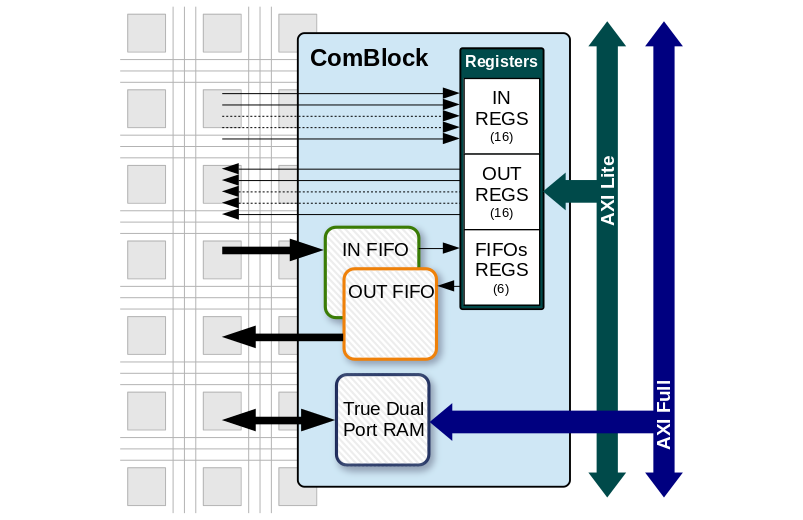
\includegraphics[width=1.0\textwidth, trim={2cm 0 2cm 0}, clip]{../images/comblock.png}
  \end{columns}
\end{frame}

%%%%%%%%%%%%%%%%%%%%%%%%%%%%%%%%%%%%%%%%%%%%%%%%%%%%%%%%%%%%%%%%%%%%%%%%%%%%%%%

\begin{frame}{Features}
  \begin{columns}
    \column{0.3\textwidth}
      \center
      
\includegraphics[width=1.0\textwidth, trim={9cm 0 9cm 0}, clip]{../images/component.png}
    \column{0.7\textwidth}
      \begin{itemize}
        \scriptsize
        \item[•] Designed with the goal of being easy to use and portable.
        \item[•] Highly configurable: 5 interfaces, which could be individually enabled, with their own parameters.
        \item[•] 0 to 16 input and output registers (configurable up to 32 bits).
        \item[•] A True Dual-Port RAM, which provides a Simple RAM interface available to the user. Its inclusion, the data width, the address width and the memory depth can be configured.
        \item[•] Two asynchronous FIFOs, one from PL to PS and another from PS to PL, with flags of empty/full, almost empty/full and underflow/overflow conditions. Their individual inclusion, the data width and the memory depth can be configured, as well as the difference to indicate almost Empty/Full.
        \item[•] Packaged for Vivado with AXI interfaces.
        \item[•] A C-Driver for the Processor side is provided.
      \end{itemize}
  \end{columns}
  \vspace{5mm}
  \tiny\center
  Under the hood, it was descripted using VHDL'93 and inferred memories of the FPGALIB project (\url{https://github.com/INTI-CMNB-FPGA/fpga_lib}), which were tested with Xilinx, Intel/Altera and Microsemi devices.
\end{frame}

%%%%%%%%%%%%%%%%%%%%%%%%%%%%%%%%%%%%%%%%%%%%%%%%%%%%%%%%%%%%%%%%%%%%%%%%%%%%%%%

\begin{frame}{Getting ComBlock}
  \begin{itemize}
    \scriptsize
    \item[•] Gitlab repository \url{https://gitlab.com/rodrigomelo9/core-comblock}
    \item[•] You can \textbf{clone} it (Git) or \textbf{download} it (compressed)
  \end{itemize}
  \center
  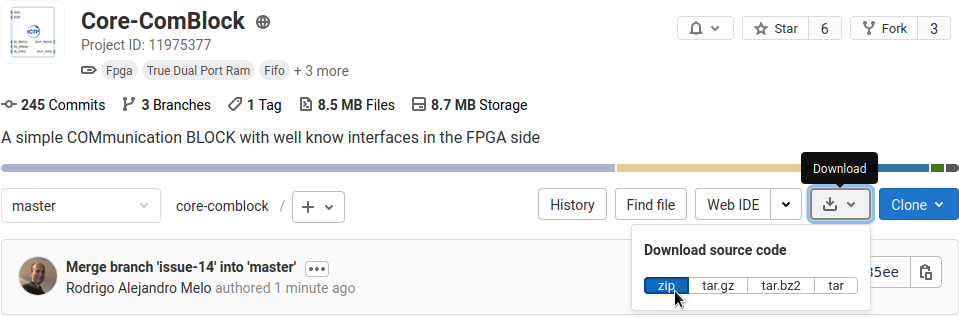
\includegraphics[width=0.9\textwidth]{../images/repo.png}
  \begin{itemize}
    \scriptsize
    \item[•] It is licensed under the BSD 3-clause.
  \end{itemize}
\end{frame}

%%%%%%%%%%%%%%%%%%%%%%%%%%%%%%%%%%%%%%%%%%%%%%%%%%%%%%%%%%%%%%%%%%%%%%%%%%%%%%%

\begin{frame}{Adding to Vivado}
  \begin{itemize}
    \scriptsize
    \item[•] Flow Navigator $\rightarrow$ Project Settings
    \item[•] IP $\rightarrow$ Repository $\rightarrow$ Add Repository button (+)
    \item[•] Browse to \textit{<COMBLOCK\_PATH>/src} $\rightarrow$ OK
  \end{itemize}
  \center
  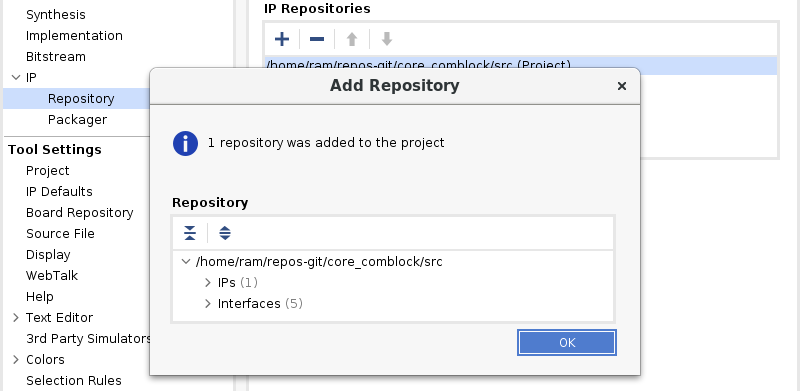
\includegraphics[width=0.6\textwidth]{../vivado/guide/add-repo.png} \\
  \tiny
  Note: the five interfaces in the image are internally used by the core.
\end{frame}

%%%%%%%%%%%%%%%%%%%%%%%%%%%%%%%%%%%%%%%%%%%%%%%%%%%%%%%%%%%%%%%%%%%%%%%%%%%%%%%

\begin{frame}{Customizations}
  \begin{columns}
    \column{0.4\textwidth}
      \begin{itemize}
        \item[•] Each user interfaces can be individually enabled, which determines the editable configurations.
        \item[•] The AXIL interface is available if at least one register or FIFO interface is used.
        \item[•] The AXIF interface is only available when the RAM interface is used.
      \end{itemize}
    \column{0.6\textwidth}
      \center
      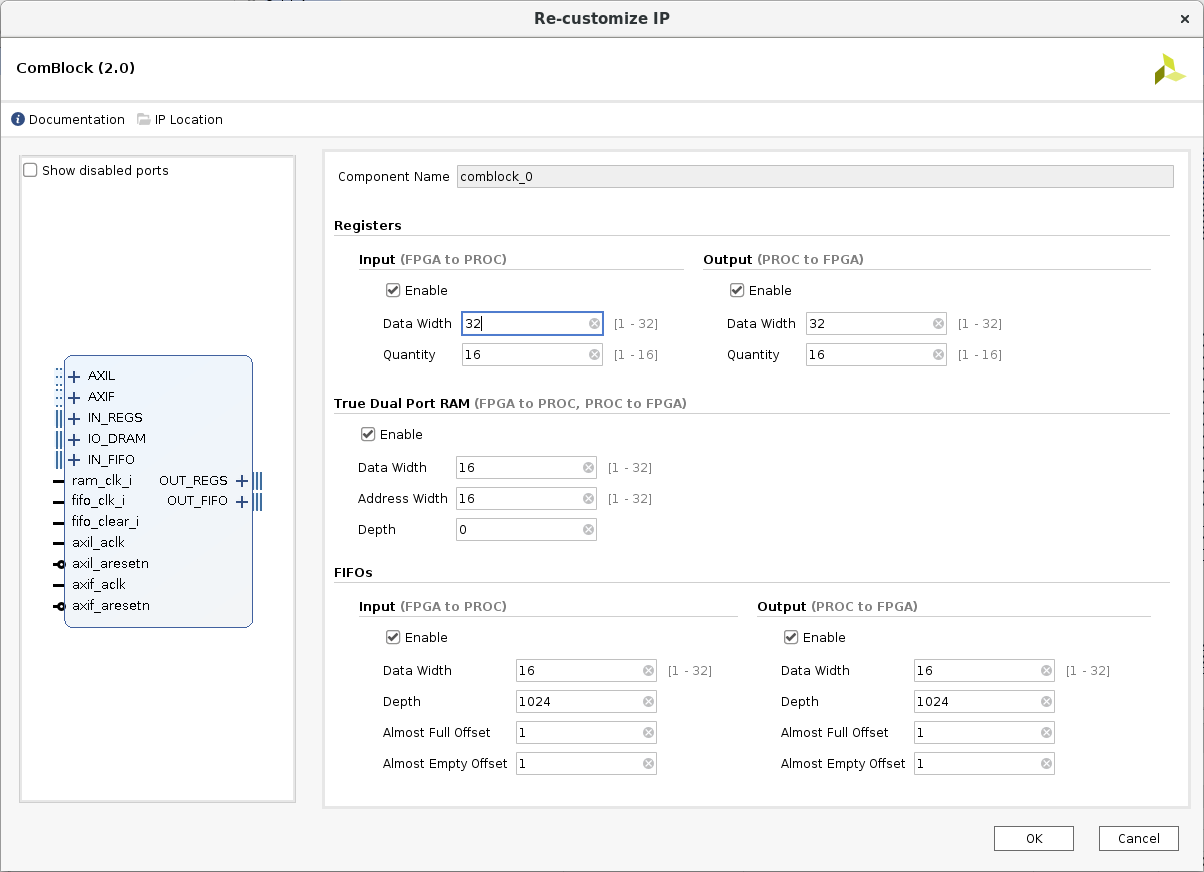
\includegraphics[width=1.0\textwidth]{../vivado/guide/config.png}
  \end{columns}
\end{frame}

\begin{frame}{Registers}
  \center
  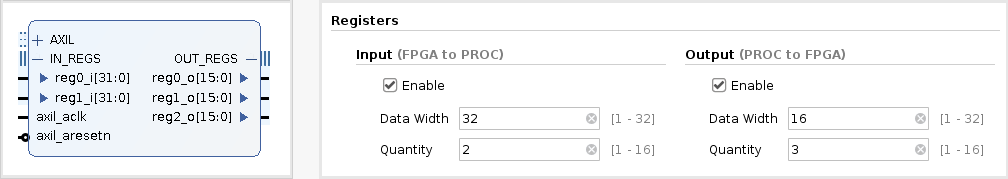
\includegraphics[width=0.9\textwidth]{../vivado/guide/only-regs.png}
  \begin{itemize}
    \item[•] Input registers are Read from 0 to 15.
    \item[•] Output registers can be Written/Read from 16 to 31.
  \end{itemize}
\end{frame}

\begin{frame}{True Dual Port RAM}
  \center
  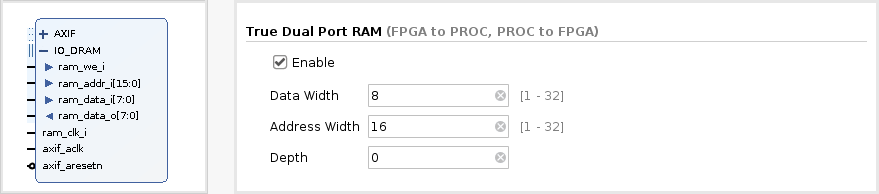
\includegraphics[width=0.9\textwidth]{../vivado/guide/only-dram.png}
  \begin{itemize}
    \item[•] The True Dual Port RAM Interface is considered as I/O (bidirectional).
    \item[•] If DEPTH is 0, the quantity of memory positions is calculated as 2**AWIDTH.
    \item[•] A DEPTH greater than 0 is useful when the complete address space produce a waste of resources (as example, in the Xilinx 7-series, the BRAM are used as 18/36 Kb, which are not a power of 2).
    \item[•] Due to its nature, is a good interface to perform a Clock Domain Crossing (CDC).
  \end{itemize}
\end{frame}

\begin{frame}{FIFOs}
  \center
  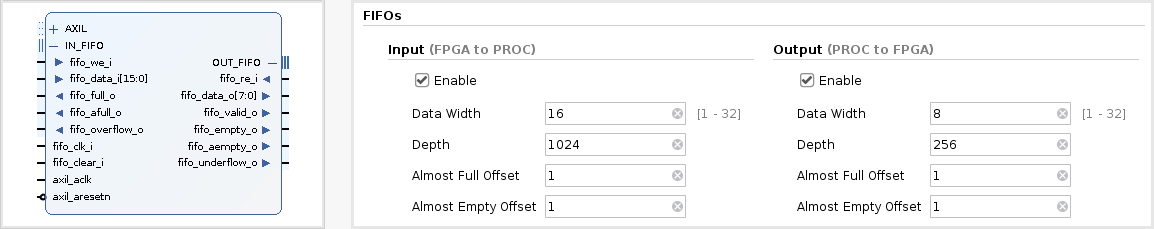
\includegraphics[width=0.8\textwidth]{../vivado/guide/only-fifos.png}
  \begin{itemize}
    \item[•] Both FIFOs are asynchronous, so they could be also used to perform a CDC.
    \item[•] The Clear input is used to have a know state in both sides of the FIFOs.
    \item[•] DEPTH has the same sense that in the DRAM\_IO interface.
    \item[•] AEMPTY and AFULL means \textit{Almost}
    \item[•] Overflow/Underflow conditions must be avoided reading Full/Empty flags to ensure not to lose data.
  \end{itemize}
\end{frame}

%%%%%%%%%%%%%%%%%%%%%%%%%%%%%%%%%%%%%%%%%%%%%%%%%%%%%%%%%%%%%%%%%%%%%%%%%%%%%%%

\begin{frame}{Registers Maps (PS side)}
  \begin{columns}
    \column{0.3\textwidth}
      \begin{itemize}
        \scriptsize
        \item[•] \textit{IN\_REGS} are available from 0 to 15 (only read).
        \item[•] \textit{OUT\_REGS} are available from 16 to 31 (read/write).
        \item[•] \textit{IN\_FIFO} registers for value, control and status are available from 32 to 34.
        \item[•] \textit{OUT\_FIFO} registers for value, control and status are available from 36 to 38.
      \end{itemize}
    \column{0.7\textwidth}
      \center
      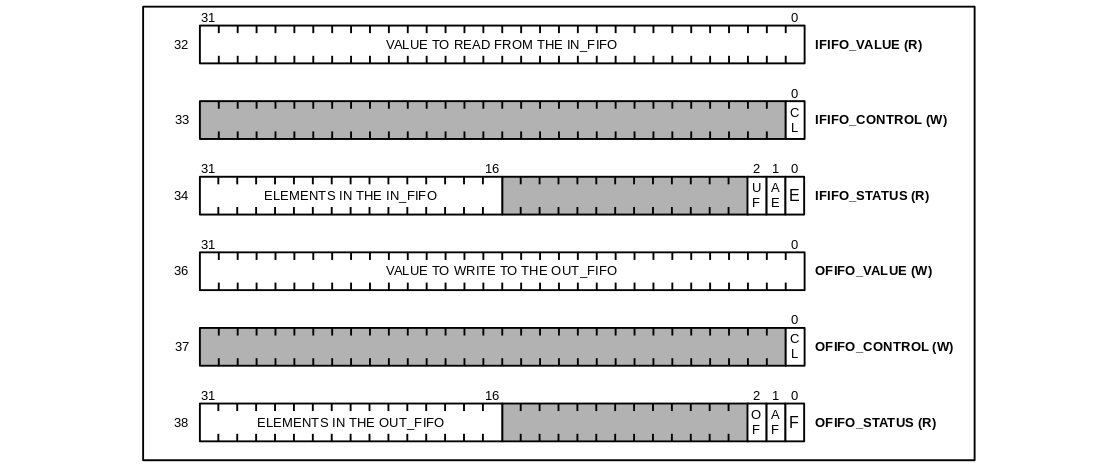
\includegraphics[width=1.0\textwidth, trim={2cm 0 2cm 0}, clip]{../images/fifo_regs.png}
  \end{columns}
\end{frame}

\begin{frame}[fragile]{C Driver}

  A C driver to be used with a Baremetal or FReeRTos project is provided:
  \begin{lstlisting}[language=C, numbers=none, basicstyle=\scriptsize]
#include "comblock.h"
  \end{lstlisting}

  The registers can be accessed by number or with the following provided \textbf{defines}:
  \begin{itemize}
    \scriptsize
    \item[•] \textit{CB\_IREGn} (0:15): Input Register 0..15
    \item[•] \textit{CB\_OREGn} (16:31): Output Register 16..31
    \item[•] \textit{CB\_IFIFO\_VALUE} (32) : \textit{IN\_FIFO} value
    \item[•] \textit{CB\_IFIFO\_CONTROL} (33) : \textit{IN\_FIFO} control
    \item[•] \textit{CB\_IFIFO\_STATUS} (34): \textit{IN\_FIFO} status
    \item[•] \textit{CB\_OFIFO\_VALUE} (36): \textit{OUT\_FIFO} value
    \item[•] \textit{CB\_OFIFO\_CONTROL} (37) : \textit{OUT\_FIFO} control
    \item[•] \textit{CB\_OFIFO\_STATUS} (38) : \textit{OUT\_FIFO} status
  \end{itemize}
\end{frame}

\begin{frame}[fragile]{Read/Write functions}
  To write/read one memory position:
  \begin{lstlisting}[language=C, numbers=none, basicstyle=\scriptsize]
void cbWrite(UINTPTR baseaddr, u32 reg, u32 value)
u32 cbRead(UINTPTR baseaddr, u32 reg)
  \end{lstlisting}
To write/read several contiguous memory positions:
  \begin{lstlisting}[language=C, numbers=none, basicstyle=\scriptsize]
void cbWriteBulk(UINTPTR baseaddr, int *buffer, u32 depth)
void cbReadBulk(int *buffer, UINTPTR baseaddr, u32 depth)
  \end{lstlisting}
Vitis/SDK, provides a file called \textit{xparameters.h}, where the base addresses of the buses are defined. Additionally, in case of the ComBlock, you can find also \textbf{defines} related to the configuration values selected in the programmable side.
\end{frame}

%%%%%%%%%%%%%%%%%%%%%%%%%%%%%%%%%%%%%%%%%%%%%%%%%%%%%%%%%%%%%%%%%%%%%%%%%%%%%%%

\begin{frame}[fragile]{Example: R/W Registers}
Write an specific Output Register:
  \begin{lstlisting}[language=C, numbers=none, basicstyle=\scriptsize]
cbWrite(AXIL_BASEADDR, CB_OREG0, 0x99);
  \end{lstlisting}
Write 16 Output Registers (option 1):
  \begin{lstlisting}[language=C, numbers=none, basicstyle=\scriptsize]
for (i=0; i < 16; i++)
    cbWrite(AXIL_BASEADDR, CB_OREG0 + i, 0x22);
  \end{lstlisting}
Write 16 Output Registers (option 2):
  \begin{lstlisting}[language=C, numbers=none, basicstyle=\scriptsize]
cbWriteBulk(AXIL_BASEADDR, wr_buffer, 16);
  \end{lstlisting}
Read an specific Input Register:
  \begin{lstlisting}[language=C, numbers=none, basicstyle=\scriptsize]
data = cbRead(AXIL_BASEADDR, CB_IREG4);
  \end{lstlisting}
\end{frame}

\begin{frame}[fragile]{Example: R/W Memories}
Write 1024 DRAM memory positions:
  \begin{lstlisting}[language=C, numbers=none, basicstyle=\scriptsize]
cbWriteBulk(AXIF_BASEADDR, wr_buffer, 1024);
  \end{lstlisting}
Read 90 DRAM memory positions:
  \begin{lstlisting}[language=C, numbers=none, basicstyle=\scriptsize]
cbReadBulk(rd_buffer, AXIF_BASEADDR, 90);
  \end{lstlisting}
Write 100 values to the Output FIFO:
  \begin{lstlisting}[language=C, numbers=none, basicstyle=\scriptsize]
for (i=0; i < 100; i++)
    cbWrite(AXIL_BASEADDR,CB_OFIFO_VALUE,i);
  \end{lstlisting}
Read 50 values from the Input FIFO:
  \begin{lstlisting}[language=C, numbers=none, basicstyle=\scriptsize]
for (i=0; i < 50; i++) {
    data[i] = cbRead(AXIL_BASEADDR, CB_IFIFO_VALUE);
  \end{lstlisting}
  \textbf{WARNING}: bulk functions can't be used with the FIFOs.
\end{frame}

%%%%%%%%%%%%%%%%%%%%%%%%%%%%%%%%%%%%%%%%%%%%%%%%%%%%%%%%%%%%%%%%%%%%%%%%%%%%%%%

\begin{frame}{Other repository resources}
  \begin{columns}
    \column{0.5\textwidth}
      \begin{itemize}
        \item[•] User Guide (\textit{doc/user\_guide.md})
        \item[•] Vivado tutorial (\textit{doc/tutorial\_vivado.md}), with SDK and Vitis step-by-step instructions.
        \item[•] Examples: test and measurement (using PyFPGA)
        \item[•] Simulations (based on cocotb)
      \end{itemize}
    \column{0.5\textwidth}
      \center
      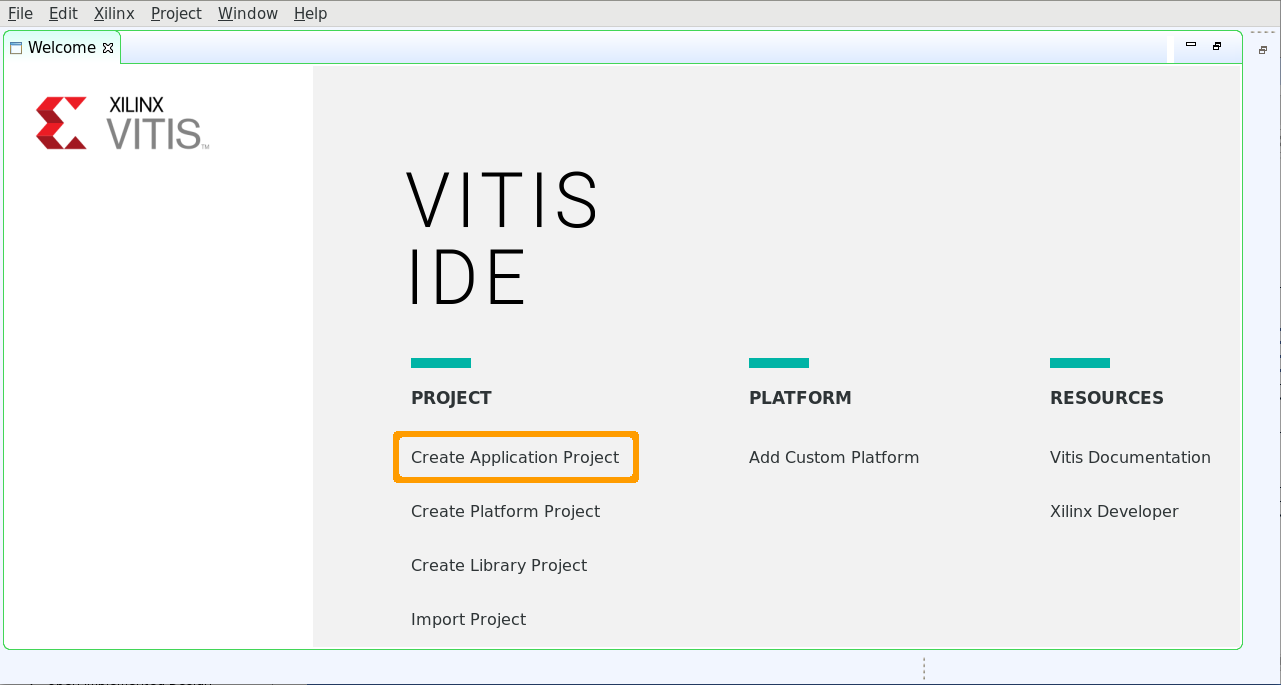
\includegraphics[width=1.0\textwidth]{../vivado/tuto/20-3.png}
  \end{columns}
\end{frame}

%%%%%%%%%%%%%%%%%%%%%%%%%%%%%%%%%%%%%%%%%%%%%%%%%%%%%%%%%%%%%%%%%%%%%%%%%%%%%%%

\begin{frame}{License}
  This presentation is distributed under a
  \textbf{Creative Commons Attribution 4.0 International License}
  (\url{https://creativecommons.org/licenses/by/4.0/}).
\end{frame}

\end{document}
